\pdfoutput=1

\documentclass[11pt]{report}
\usepackage[utf8]{inputenc}
\usepackage[T1]{fontenc}
\usepackage[Glenn]{fncychap} %Conny, Glenn, Bjarne, Bjornstrup, Rejne, Lenny
\usepackage[top=0.5cm, bottom=2cm, left=2cm , right=2cm]{geometry}
\usepackage{graphicx}
\usepackage{fourier}
\usepackage[frenchb]{babel}
\usepackage{color}
\usepackage{pifont}
\usepackage{framed}
\usepackage{booktabs}
\definecolor{forestgreen}{rgb}{0.13,0.54,0.13}

%%% Custom headers/footers (fancyhdr package)
\usepackage{fancyhdr}
\pagestyle{fancyplain}
\fancyhead{}                                            % No page header
\fancyfoot[L]{}                                         % Empty
\fancyfoot[C]{}                                         % Empty
\fancyfoot[R]{\thepage}                                 % Pagenumbering
\renewcommand{\headrulewidth}{0pt}          % Remove header underlines
\renewcommand{\footrulewidth}{0pt}              % Remove footer underlines
\setlength{\headheight}{13.6pt}


%%% Maketitle metadata
\newcommand{\horrule}[1]{\rule{\linewidth}{#1}}     % Horizontal rule

\title{
        %\vspace{-1in}
        \usefont{OT1}{bch}{b}{n}
        \normalfont \normalsize \textsc{Université Catholique de Louvain-La-Neuve } \\ [25pt]
        \horrule{0.5pt} \\[0.4cm]
        \huge \emph{Notes de cours - Circuits et mesures - LELEC1370} \\
        \horrule{2pt} \\[0.5cm]
}
\author{
        \normalfont                                 \normalsize
            \normalsize
    AMANPREET SINGH\\
        Dimanche 21 février, 2015 \\\\
}
\date{}
\begin{document}
\maketitle
\newpage

\tableofcontents
\textcolor{forestgreen}{\chapter{Les circuits résistifs}}
\section{Définitions}
Liste des définitions mathématiques de phénomènes physiques :
\begin{framed}
\ding{43} Tension : $v = \frac{dw}{dq}$ \left[ V \right]  \newline

\ding{43} Courant : $i = \frac{dq}{dt}$ \left[ A \right] \newline

\ding{43} Puissance : $p = vi = \frac{dw}{dq}\frac{dq}{dt} = \frac{dw}{dt}$ \left[ W \right] \newline

\ding{43} Energie : $\Delta w = \int _{ { t }_{ 1 } }^{ { t }_{ 2 } }{ p\hspace{0.3mm}dt } = \int _{ { t }_{ 1 } }^{ { t }_{ 2 } }{ vi\hspace{0.3mm}dt } $ \left[ J \right]
\end{framed}
\section{Conventions}
Cette section explique la convention utilisé pour déterminer le signe du courant et d'une tension :
\begin{framed}
  \ding{43} Le signe du courant est défini selon le sens de circulation du courant. Celui-ci est défini comme étant positif (charges positives) si le courant rentre dans l'élément du circuit par la borne positive du dipôle.\newline

  \ding{43} La borne positive et négative du dipôle est choisi de manière arbitraire mais une fois qu'elle est défini, elle ne doit plus changer pour les calculs.\newline

  \ding{43} La puissance est soit absorbée ou fournie. Par convention, une puissance absorbée est positive et une puissance fournie est négative. De plus dans un circuit résistif, il est intéressant de vérifier que $\sum { p } =0$ car cette condition est toujours vraie.\\

  Pour une résistance, la puissance est toujours positive \newline
  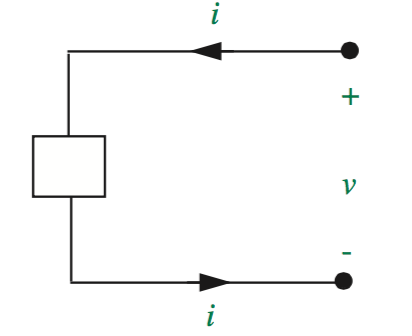
\includegraphics[width=3cm]{1.png}

\end{framed}
\newpage
\section{Les éléments d'un circuit résistif}
Les éléments d'un circuit résistif idéaux (sans résistances internes)
\begin{framed}
  \ding{43} Source de tension et courant indépendantes : \newline
  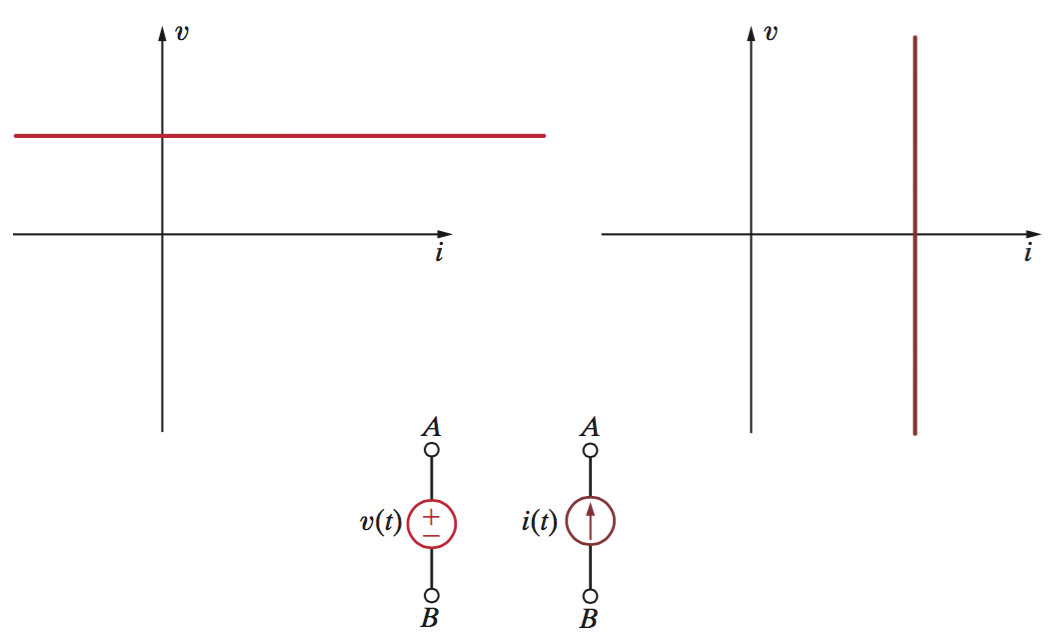
\includegraphics[width=7cm]{2.png}\newline

  \ding{43} Source de tension et courant dépendantes commandées en tension ou courant : \newline
  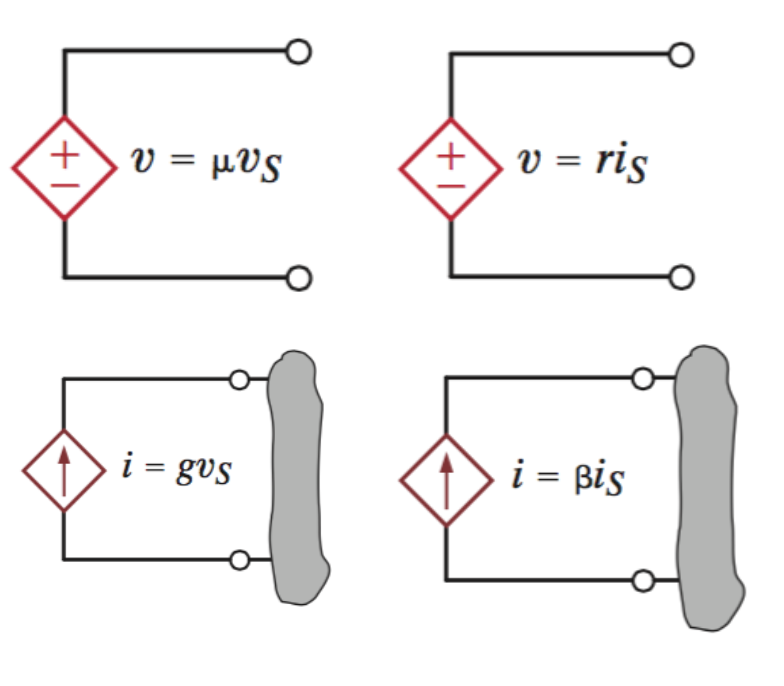
\includegraphics[width=7cm]{3.png}\newline

  \ding{43} Une résistance est liée par sa tension et son courant par la relation d'Ohm : $v = iR$ et R est mesurée en Ohm $\left[ \Omega \right]$ \newline
  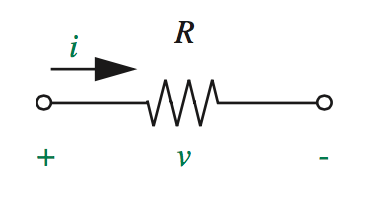
\includegraphics[width=3cm]{6.png}\newline

  \ding{43} La conductance est définie comme étant l'inverse d'un résistance : $G = \frac{1}{R}$  $\left[ S \right]$  et donc $i = Gv$ $ \left[ A \right]$ \newline

  \ding{43} $p = \frac{v^2}{R} = i^2R = \frac{i^2}{G} = Gv^2$ \newline

  \ding{43} Pour une résistance linéaire, la relation v-i est .. linéaire : \newline
  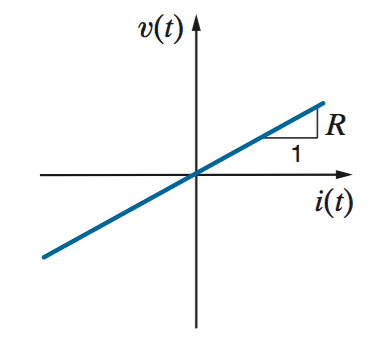
\includegraphics[width=4cm]{4.png}

\end{framed}

\section{Simplifications de résistances et circuits types}
Cette section présente des techniques qui permettent des simplifier un réseau de résistances en un circuit plus simple et équivalent.
\begin{framed}
  \ding{43} Résistances en séries : ${ R }_{ eq }=\sum { { R }_{ i } }$ et les courants sont les mêmes car en séries.\newline

  \ding{43} Résistances en parallèles : $\frac { 1 }{ { R }_{ eq } } =\sum { \frac { 1 }{ { R }_{ i } }  } $ ou ${ R }_{ eq }=\frac { 1 }{ \sum { { G }_{ i } }  } $ et les tensiosn sont les mêmes car en parallèles.\newline

\end{framed}

\section{CC et CO}
Cette section a pour but d'expliquer les notions de court-circuit et circuit ouvert.
\begin{framed}
  \ding{43} Un court-circuit (cas b) est un élément à travers lequel la différence de potentiels est nulle, peu importe le courant traversant l'élément. L'élément se comporte comme une résistance linéaire quand $R\rightarrow 0 $\newline

  \ding{43} Un circuit ouvert (cas c) est un élément à travers lequel aucun courant ne passe, peu importe la différence de potentiel entre les 2 bornes. L'élément se comporte comme une résistance linéaire quand $R\rightarrow \infty $\newline
      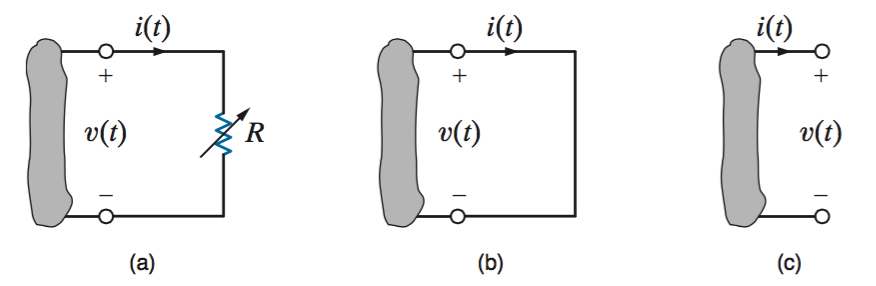
\includegraphics[width=10cm]{5.png}

\end{framed}

\section{KCL et KVL}
Cette section présente une technique d'analyse des courants et tensions dans un circuit résistif.
Elles se démontrent facilement en utilisant les équations de Maxwell et en prennant les hypothèses $\frac{d\phi}{dt} = 0$ et $\frac{dq}{dt} = 0$
\begin{framed}
  \ding{43} KCL : $\sum { { i }_{ in } } = \sum { { i }_{ out } }$, les inconnues sont des tensions. \newline

  \ding{43} Diviseur de courants, formule dérivée de KCL : ${ i }_{ { R }_{ i } }=i\frac { { G }_{ i } }{ \sum _{ i=1 }^{ n }{ { G }_{ i } }  } $\newline
  Utilisée lorsque qu'on a une source de courant en parallèle avec des résistances en parallèles.\newline

  \ding{43} KVL : $\sum { v } = 0$, les inconnues sont des courants. \newline

  \ding{43} Diviseur de tensions, formule dérivée de KVL : ${ v }_{ { R }_{ i } }=v\frac { { R }_{ i } }{ \sum _{ i=1 }^{ n }{ { R }_{ i } }  }$\newline
  Utilisée lorsque qu'on a une source de tension en série avec des résistances en séries.\newline
\end{framed}
\newpage
\section{Circuits types}
Cette section présente les différents types de circuits résistifs intéressants à résoudre (voir exercices)
\begin{framed}
  \ding{43} Formules dualité triangles/étoiles : \newline
  ${ R }_{ a }=\frac { { R }_{ 1 }{ R }_{ 2 } }{ { R }_{ 1 }+{ R }_{ 2 }+{ R }_{ 3 } }$ \newline
  $ { R }_{ b }=\frac { { R }_{ 2 }{ R }_{ 3 } }{ { R }_{ 1 }+{ R }_{ 2 }+{ R }_{ 3 } }$ \newline
  ${ R }_{ c }=\frac { { R }_{ 1 }{ R }_{ 3 } }{ { R }_{ 1 }+{ R }_{ 2 }+{ R }_{ 3 } }$ \newline
 Si $R_1=R_2=R_3$ et $R_a=R_b=R_c$, alors ${ R }_{ \Delta  }={ 3R }_{ Y }$\newline
 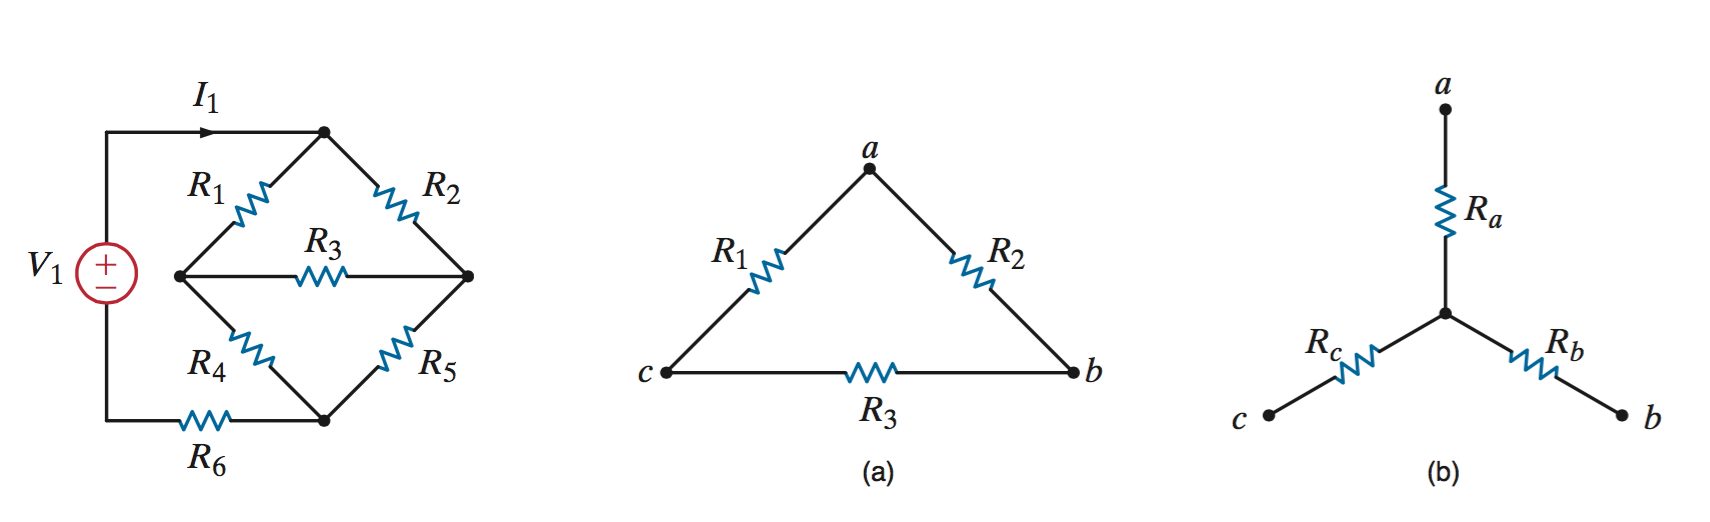
\includegraphics[width=14cm]{7.png}\newline
 \ding{43} Circuit en échelle, transistor à effet de champ, pont de Wheatstone, etc.
\end{framed}
\section{Equivalences entre circuits}
Cette section présente comment simplifier des sources de courants, tensions et des résistances
\begin{framed}
   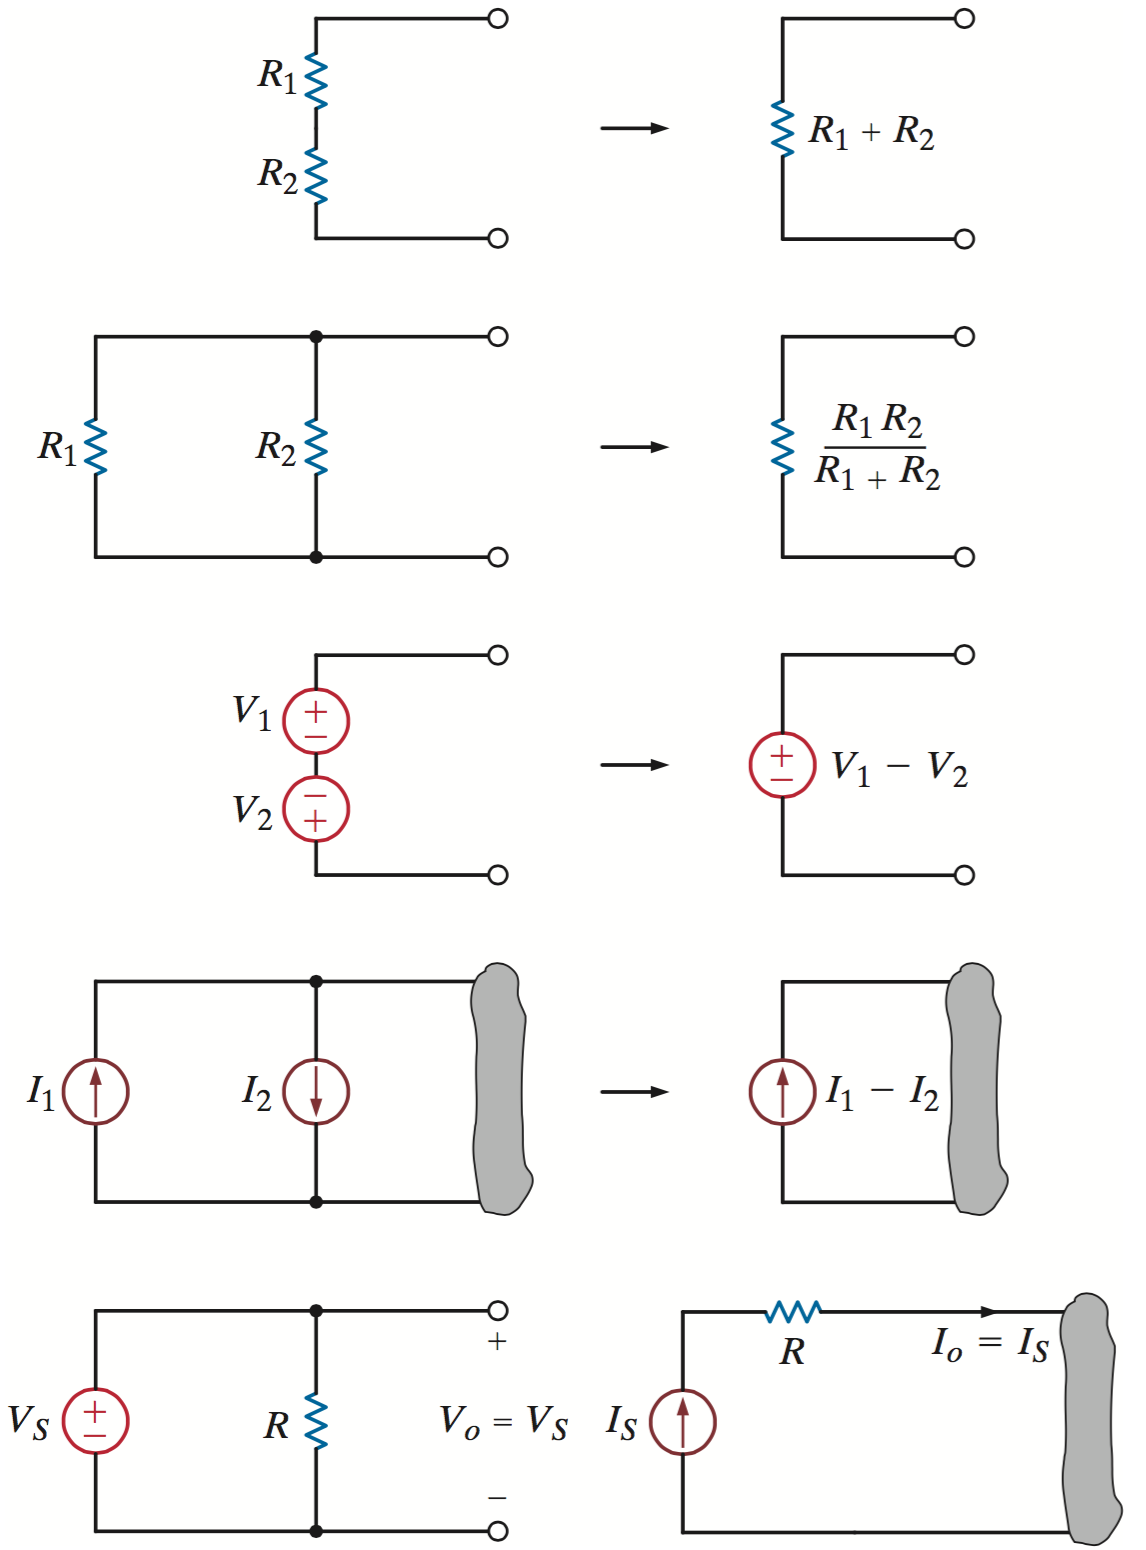
\includegraphics[width=8cm]{8.png}\newline
\end{framed}

\textcolor{forestgreen}{\chapter{Les techniques d'analyse de circuits}}
\section{introduction}
Il existe plusieurs méthodes pour trouver des courants et des tensions dans des circuits électriques. \\
Ces notes de cours présentent la méthode des noeuds, la méthode des branches, le principe de superposition et les équivalents de thévenins et norton.
\section{Méthode des noeuds}
\begin{framed}

\end{framed}
\section{Méthode des branches}
\begin{framed}

\end{framed}
\section{Principe de superposition}
\begin{framed}

\end{framed}
\section{Equivalents de thévenins et norton}
\begin{framed}

\end{framed}

\textcolor{forestgreen}{\chapter{Circuits en régime sinusoidal}}
\section{Circuit capacitif et inductif}
Section qui présente les caractéristiques d'un circuit capacitif (RC) et inductif (RL) : \newline
\begin{framed}
  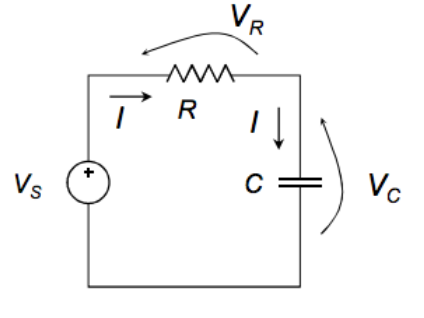
\includegraphics[width=4cm]{9.png}\newline

  \ding{43} Equation constitutif de la capacité :  $I(t) = C\frac{dV_c(t)}{dt}$\newline

  \ding{43} KVL : $-V_s + V_R + V_c = 0$ \newline

  \ding{43} Eléments en séries : $I(t) = \frac{V_s(t)-V-c(t)}{R}$\newline

  \ding{43} Equation différentielle : $RC\frac{dV_c(t)}{dt} + V_c(t) = -V_s(t)$\newline

  \ding{43} Constante de temps : $\tau = RC$\newline

  \ding{43} Solution : $V_c(t) = A + Be^{-t/\tau}$\newline

  \ding{43} CI : $V_c(t=0) = A + B$\newline

  \ding{43} CF = $V_c(t=\infty) = A$\newline
\end{framed}
\newpage
\begin{framed}
  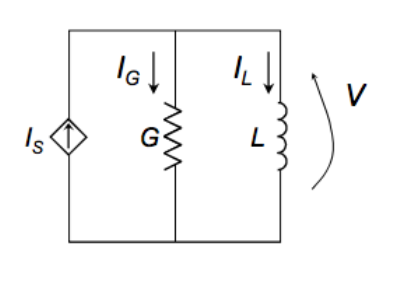
\includegraphics[width=4cm]{10.png}\newline

  \ding{43} Equation constitutif de l'inductance :  $I(t) = L\frac{dI_L(t)}{dt}$\newline

  \ding{43} KCL : $I_S(t) = I_G(t) + I_L(t)$ \newline

  \ding{43} Eléments en parallèles : $V = \frac{I_G}{G}$\newline

  \ding{43} Equation différentielle : $GL\frac{dI_L(t)}{dt} + I_L(t) = -I_s(t)$\newline

  \ding{43} Constante de temps : $\tau = GL$\newline

  \ding{43} Solution : $I_L(t) = A + Be^{-t/\tau}$\newline

  \ding{43} CI : $I_L(t=0) = A + B$\newline

  \ding{43} CF = $I_L(t=\infty) = A$\newline

\end{framed}
\section{Signal sinusoïdal}
Un signal sinusoïdal est une fonction d'un cosinus ou d'un sinus à une certaine fréquence. Il peut être aussi une combinaison linéaire (CL) d'un sinus et cosinus.
\begin{framed}
  \ding{43} Fréquence : $f = \frac{1}{T}$\newline

  \ding{43} Période : $T = \frac{1}{f}$\newline

  \ding{43} Fréquence angulaire : $\omega = \frac{2\pi}{T} = 2\pi f$\newline

  \ding{43} Fonction cosinus d'amplitude $a_c$ et fréquence $\omega t$ : $f_{cosinus} = a_ccos(\omega t)$\newline

  \ding{43} Fonction sinus d'amplitude $a_s$ et fréquence $\omega t$ : $f_{sinus} = a_ssin(\omega t)$\newline

  \ding{43} Propriété trigonométrique : $f_{sinus} = a_ssin(\omega t) =  a_scos(\omega t - \frac{\pi}{2})$\newline

  \ding{43} Fonction CL d'amplitude $a_{CL}$ et fréquence $\omega t$ : $f_{CL} = a_ccos(\omega t) + a_ssin(\omega t)$\newline

  \ding{43}  Fonction CL exprimé en fonction d'un cosinus et d'un déphasage : $\frac{a_c}{cos(\phi)}cos(\omega t -\phi)$\newline

  \ding{43} Déphasage compris entre $\frac{-\pi}{2}$ et  $\frac{\pi}{2}$  d'une fonction CL : $\phi = tan^{-1} (\frac{a_s}{a_c})$\newline

\end{framed}


\textcolor{forestgreen}{\chapter{Analyse sinusoïdale en régime permanent}}
\section{Signal sinusoïdal}
Un signal sinusoïdal est une fonction qui dépend d'un cos, d'un sin ou d'une combinaisons des deux. \\
Ce signal est à une certaine fréquence, une certaine amplitude et peut être déphasé.\\
Un sin est après tout qu'un cos qui est déphasé de $- 90^{\circ}$

\begin{framed}
  \ding{43} Fréquence : $f = \frac{1}{T} \left[ Hz \right]$ \newline

  \ding{43} Période : $T= \frac{1}{f} \left[ s \right]$ \newline

  \ding{43} Fréquence angulaire : $\omega = \frac{2\pi}{T} = 2\pi f \left[ rad.s^{-1} \right]$ \newline

  \ding{43} Source de tension : $v(t) = V_mcos(\omega t + \phi)$ \newline

  \ding{43} Source de courant : $i(t) = I_mcos(\omega t + \phi)$ \newline

  \ding{43} Retard (delay, à ne pas confondre avec constante de temps !) : $\tau = \frac{\phi}{\omega} \left[ s \right]$ \newline

  \ding{43} Tension effective : $V_{RMS} = \frac{V_m}{\sqrt{2}}$ \newline

  \ding{43} Conversion rad <-> deg : $\theta_{deg} = \theta_{rad}\frac{180}{\pi}$ \newline

  \ding{43} Propriété trigonométrique : $sin(\theta) = cos(\theta - 90^{\circ})$\newline

  \ding{43} Fréquence propre : $\omega_0 = \frac{1}{\tau}$\newline

  \ding{43} Déphasage en régime permanent : $\phi = tan^{-1}(-\frac{\omega}{\omega_0})$ \newline

  \ding{43} Constante de temps circuit RC : $\tau = RC$  \newline

  \ding{43} Constante de temps circuit RL : $\tau = \frac{L}{R}$ \newline

  \ding{43} Constante de temps circuit RLC : $\tau = $ \newline


\end{framed}
\newpage

\section{Signal de sorti dans le domaine temporel suite à un signal sinusoïdal en entrée}
Dans le domaine temporelle, nous pouvons calculer la tension/courant de sortie en fonction d'une source sinusoïdale. Il s'agit en général, la solution d'une équation différentielle du circuit en utilisant des conditions initiales.

\begin{framed}
  \ding{43} $v_{out} =$ (atténuation) * $\left[ (transitoire) + (déphasage) \right]$ \newline

  \ding{43} Régime permanent si : $(transitoire) \rightarrow 0$ lorsque $t >> \tau$ et $V_{out} (t +P) = V_{out} (t)$ $\forall t$ \newline

  \ding{43} Equation différentielle : $\frac{1}{\omega_0}\frac{dv_{out}(t)}{dt} + v_{out}(t) = V_{m}cos(\omega t)$\newline

  \ding{43} Solution dans le domaine temporelle : $v_{out}(t) = kV_m  \left[ T(t) + cos(\omega t +\phi) \right]$ \newline

  \ding{43} Solution en régime permanent uniquement : $v_{out}(t) = kV_m  \left[cos(\omega t +\phi) \right]$ \newline
\end{framed}

\section{Hypothèses prises en compte pour la solution général}
Le signal de sorti est solution d'une équation différentielle qui dépend du signal d'entrée mais la solution en régime est valable que sous certaines conditions :
\begin{framed}
  \ding{43} La réponse (en régime) à une excitation sinusoïdale est une sinusoïde atténuée et déphasée de même fréquence (isomorphe à l'excitation). \newline

  \ding{43} La solution générale dans le domaine temporelle est valable si seulement le circuit est stable, c'est-à-dire que le terme transitoire et toutes ses dérivées tendent vers 0 pour t grand et si les sources indépendantes sont nulles, tous les courants et tensions tendent vers 0 pour t grand.\newline

  \ding{43} Valable pour un circuit :  linéaire, ne contenant qu'une source indépendante (sinon voir superposition), dont la source est une sinusoïde de fréquence $\frac{\omega}{2\pi}$, en état de régime.\newline

  \ding{43} Les signaux dépendants sont tous de la même forme que la source, à la même fréquence, avec une amplitude différente et avec une phase différente. \newline

  \ding{43} Les signaux peuvent être représentés par un phaseur, qui contient uniqument les informations d'amplitude et de phase. \newline


\end{framed}
\newpage
\section{Représentation phasorielle}
Pour faciliter les calculs, nous pouvons passer d'une expresion $v(t)$ ou $i(t)$ à une expression $v(\phi)$ ou $i(\phi)$.\\
La dérivation et l'intégration deviennent de simple produit, les équations différentielles et les intégrales deviennent des équations algébriques :

\begin{framed}
  \ding{43} Phaseur qui représente une tension : $V = V_Me^{j\phi}$\newline

  \ding{43} Phaseur qui représente une tension : $I = I_Me^{j\phi}$\newline

  \ding{43} $j = \sqrt{-1}$\newline

  \ding{43} $e^{+- j\phi} = cos(\phi) +- jsin(\phi)$\newline

  \ding{43} Forme rectangulaire, facilite addition et soustraction : $V = V_me^{j\phi} = V_m\left[ cos(\phi) + jsin(\phi) \right]$\newline

  \ding{43} Forme polaire, facilite multiplication et division : $V = V_me^{j\phi} = V_m\angle \phi$\newline

  \ding{43} $cos(\omega t + \phi) = \Re (e^{j(\omega t + \phi)})$ \newline

  \ding{43} $sin(\omega t + \phi) = \Im (e^{j(\omega t + \phi)})$ \newline

  \ding{43} De manière générale, transformation du domaine temporelle au domaine fréquentielle : \newline
  \indent $V_Mcos(\omega t + \phi) +j0 = V_Mcos(\omega t + \phi) + jV_M sin(\omega t + \phi) = \left[ V_Me^{j\phi}\right]e^{j\omega t}$\newline

  \ding{43} De manière générale, transformation du domaine fréquentielle au domaine temporelle : \newline
  \indent $\left[ V_Me^{j\phi}\right]e^{j\omega t} =  \Re (V_Me^{j(\omega t + \phi)}) = V_Mcos(\omega t + \phi)$\newline

  \ding{43} $\frac{d}{dt} \left[ Ae^{j\phi} \right]e^{j\omega t} = \left[ j\omega Ae^{j\phi} \right]e^{j\omega t} $\newline

  \ding{43} $\int { \left[ Ae^{ j\phi  } \right] e^{ j\omega t } } dt=\left[ \frac { 1 }{ j\omega  } Ae^{ j\phi  } \right] e^{ j\omega t }$\newline
\end{framed}

\section{Calculs avec les phaseurs}
Section qui présente comment calculer avec des complexes :
\begin{framed}

  \ding{43}Addition : forme rectangulaire : \\
  \indent $r_1\left[ cos(\phi_1) + jsin(\phi_1) \right] +  r_2\left[ cos(\phi_2) + jsin(\phi_2) \right] =  (r_1cos(\phi_1) + r_2cos(\phi_2)) + j(r_1sin(\phi_1) + r_2sin(\phi_2))$\newline

  \ding{43}Soustraction : forme rectangulaire : \\
  \indent $r_1\left[ cos(\phi_1) + jsin(\phi_1) \right] -  r_2\left[ cos(\phi_2) + jsin(\phi_2) \right] =  (r_1cos(\phi_1) - r_2cos(\phi_2)) + j(r_1sin(\phi_1) - r_2sin(\phi_2))$\newline

  \ding{43}Multiplication : forme polaire : $(r_1\angle \phi_1) * (r_2\angle \phi_2) = r_1r_2\angle \phi_1+\phi_2$\newline

  \ding{43}Division : forme polaire : $\frac{(r_1\angle \phi_1)}{(r_2\angle \phi_2)} = \frac{r_1}{r_2}\angle \phi_1-\phi_2$\newline

\end{framed}

\begin{table}[]
\centering
\caption{Table des formules}
\label{my-label}
\begin{tabular}{@{}|c|c|c|c|@{}}
\toprule
\textbf{ELEMENTS}          & \textbf{IMPEDANCE (Z)}           & \textbf{ADMITTANCE (Y)}           & \textbf{EQUATIONS CONSTITUTIFS} \\ \midrule
\textbf{Source de tension} & \textbf{R, si pas idéale}        & \textbf{G}                        & \textbf{$V= V_M(e^{j\psi_V})$}    \\ \midrule
\textbf{Source de courant} & \textbf{R, si pas idéale}        & \textbf{G}                        & \textbf{$I= I_M(e^{j\psi_I})$}    \\ \midrule
\textbf{Résistance}        & \textbf{R}                       & \textbf{$G=\frac{1}{R}$}                        & \textbf{$V = ZI$, $I = YV$ et $\phi=0$}   \\ \midrule
\textbf{Inductance}        & \textbf{$j\omega L$}             & \textbf{$j(\frac{-1}{\omega L})$} & \textbf{$V = ZI$, $I = YV$ et $\phi=\frac{\pi}{2}$}   \\ \midrule
\textbf{Condensateur}      & \textbf{$j(\frac{-1}{\omega C})$} & \textbf{$j\omega C$}              & \textbf{$V = ZI$, $I = YV$ et $\phi=\frac{-\pi}{2}$}   \\ \bottomrule
\end{tabular}
\end{table}
\newpage
\section{Impédances et admittance}
Définitions pour un dipôle :
\begin{framed}
  \ding{43}Impédance d'un dipôle : $V = ZI$\newline

  \ding{43}Impédance par définition : $Z = \frac{V}{I} = \frac{|V|}{|I|}e^{j(arg(V)-arg(I))} = \frac{V}{I}e^{j(\psi_V-\psi_I)}$\newline

  \ding{43}Convention : $\phi = \psi_V-\psi_I$\newline

  \ding{43}Notation polaire impédance : $Z = |Z|e^{jarg(Z)} = Ze^{j\phi}$\newline

  \ding{43}Notation cartésienne  impédance : $Z = R +jX$, avec X étant la réactance\newline

  \ding{43}Admittance d'un dipôle : $I= YV$\newline

  \ding{43}Notation polaire admittance : $Y = \frac{I}{V} = |Y|e^{jarg(Y)} = Ye^{-j\phi}$\newline

  \ding{43}Notation cartésienne admittance : $Y = G + jB$ avec G la conductance et B la susceptance\newline

  \ding{43}Relation impédance - admittance : $Z = \frac{1}{Y}$\newline

\end{framed}

\end{document}

%%% Local Variables:
%%% mode: latex
%%% TeX-PDF-mode: t
%%% End:
